\subsubsection{Phase 1: Initialisierung der Daten}

Vor der Durchführung von Tests ist es wichtig, die zu testende
Plattform mit Daten vorzubereiten. Dies ermöglicht es, die
Ausgangssituation der Plattform, die man testen möchte, zu
reproduzieren. Wenn beispielsweise die Verbindung eines Benutzers
mit einer Plattform getestet werden soll, ist es wichtig, dass die
Daten dieses Benutzers bereits in der Datenbank vorhanden sind.

Im aktuellen Fall wird dies von einem Docker-Container namens
Initializer (wird im Kapitel über Docker ausführlich behandelt)
durchgeführt, dessen Zweck  ist, ein Skript auszuführen, das Daten
in den JBoss-Server von jExam einspeist. Im Falle des
Registrierungstests wird eine gültige, aber nicht auf der
Plattform registrierte Matrikelnummer generiert (siehe \Cref{fig:testData}).

\begin{figure}[H]
    \centering
    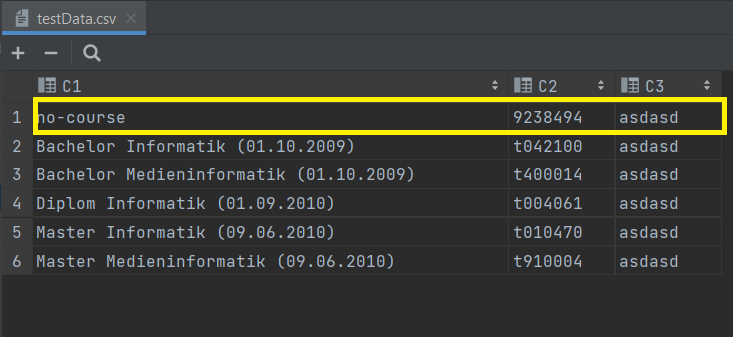
\includegraphics[scale=0.7]{images/testData}
    \caption{Vom Initializer erzeugte CSV-Daten} \label{fig:testData}
\end{figure}